\documentclass{article}
\usepackage{amsmath,amsfonts,amsthm,amssymb,amsopn,bm}
\usepackage[margin=.9in]{geometry}
\usepackage{graphicx}
\usepackage{url}
\usepackage[usenames,dvipsnames]{color}
\usepackage{fancyhdr}
\usepackage{multirow}
\usepackage{listings}
\usepackage{hyperref}
\usepackage{subfig}

\definecolor{keywords}{RGB}{255,0,90}
\definecolor{comments}{RGB}{0,0,113}
\definecolor{red}{RGB}{160,0,0}
\definecolor{green}{RGB}{0,150,0}
 
\lstset{language=Python, 
        basicstyle=\ttfamily\tiny, 
        keywordstyle=\color{keywords},
        commentstyle=\color{comments},
        stringstyle=\color{red},
        showstringspaces=false}

\newcommand{\argmax}{\arg\!\max}
\newcommand{\argmin}{\arg\!\min}
\newcommand{\field}[1]{\mathbb{#1}}
\newcommand{\1}{\mathbf{1}}
\newcommand{\E}{\mathbb{E}} 
\renewcommand{\P}{\mathbb{P}}
\newcommand{\N}{\mathcal{N}} % NormalDist
\newcommand{\R}{\field{R}} % real domain
% \newcommand{\C}{\field{C}} % complex domain
\newcommand{\F}{\field{F}} % functional domain
\newcommand{\T}{^{\textrm T}} % transpose
\def\diag{\text{diag}}

%% operator in linear algebra, functional analysis
\newcommand{\inner}[2]{#1\cdot #2}
\newcommand{\norm}[1]{\left\|#1\right\|}
\newcommand{\twonorm}[1]{\|#1\|_2^2}
% operator in functions, maps such as M: domain1 --> domain 2
\newcommand{\Map}[1]{\mathcal{#1}}
\renewcommand{\theenumi}{\alph{enumi}} 

\newcommand{\Perp}{\perp \! \! \! \perp}

\newcommand\independent{\protect\mathpalette{\protect\independenT}{\perp}}
\def\independenT#1#2{\mathrel{\rlap{$#1#2$}\mkern2mu{#1#2}}}
\newcommand{\vct}[1]{\boldsymbol{#1}} % vector
\newcommand{\mat}[1]{\boldsymbol{#1}} % matrix
\newcommand{\cst}[1]{\mathsf{#1}} % constant
\newcommand{\ProbOpr}[1]{\mathbb{#1}}
\newcommand{\points}[1]{\small\textcolor{magenta}{\emph{[#1 points]}} \normalsize}
\date{{}}

\setlength\parindent{0px}

\begin{document}
\title{Homework \#4 A}
\author{\normalsize{Spring 2020, CSE 446/546: Machine Learning}\\
\normalsize{Dino Bektesevic}}
\maketitle

Collaborated: Conor Sayers, Joachim Moeyenes, Jessica Birky, Leah Fulmer

\section*{Conceptual Questions}
A.1 The answers to these questions should be answerable without referring to external materials. Briefly justify your answers with a few words
\begin{enumerate}
    \item \points{2} True or False: Training deep neural networks requires minimizing a non-convex loss function,and therefore gradient descent might not reach the globally-optimal solution.
    \item \points{2} True or False: It is a good practice to initialize all weights to zero when training a deep neural network.
    \item \points{2} True or False: We use non-linear activation functions in a neural network’s hidden layers so that the network learns non-linear decision boundaries.
    \item \points{2}  True or False: Given a neural network, the time complexity of the backward pass step in the back-propagation algorithm can be prohibitively larger compared to the relatively low time complexity of the forward pass step.
    \item \points{2} True or False: Autoencoders, where the encoder and decoder functions are both neural networks with nonlinear activations, can capture more variance of the data in its encoded representation than PCA using the same number of dimensions.
\end{enumerate}



\section*{Think before you train}

A2. In class, we discussed some of the ways in which many datasets describing crime have various shortcomings in describing the entire landscape of illegal behavior in a city,  and that these shortcomings often fall disproportionately on minority communities. Some examples include that crimes are reported at different rates indifferent neighborhoods, that police respond differently to the same crime reported or observed in different neighborhoods, and that police spend more time patrolling in some neighborhoods than others.
\begin{enumerate}
    \item \points{5} Please describe two statistical problems arising from one or more of these issues (or others mentioned in class, or others from some other source that you cite relating to datasets compiled related to crime in the US), and what real-world implications might follow from ignoring these issues. A short paragraph for each statistical problem suffices.
    \item \points{5} For each of your previously identified statistical concerns above, propose a technical “fix” (e.g.a new sampling strategy, some training method for which few or no distributional assumptions are needed on the training set).
    \item \points{5} The solutions you described in (b) might only take you so far towards ensuring a model has similarly positive impact on different communities. Describe two reasons why a machine learning model trained to predict $f(x)$ from $x$ might have different accuracy on two different populations, even if the training data is drawn i.i.d. from the true distribution over the event of interest. [These assumptions exclude the possibility that the two populations are sampled from at rates different from their latent frequency, though their latent frequencies may be different.]
\end{enumerate}






\section*{Unsupervised Learning with Autoencoders}

A3. Last homework we used PCA to project and reconstruct data from the MNIST dataset. In this exercise, we will train two simple autoencoders to perform dimensionality reduction on MNIST. As discussed in lecture, autoencoders are a long-studied neural network architecture comprised of an encoder component to summarize the latent features of input data and a decoder component to try and reconstruct the original data from the latent features. 

\textbf{Weight Initialization and PyTorch}

Last assignment, we had you refrain from using \textbf{torch.nn} modules. For this assignment, we recommend using \textbf{nn.Linear} for your linear layers. You will not need to initialize the weights yourself; the default He/Kaiming uniform initialization in PyTorch will be sufficient for this problem. Hint: we also recommend using the nn.Sequential module to organize your network class and simplify the process of writing the forward pass. 

\textbf{Training}

Use optim.Adam for this question. Experiment with different learning rates. Use mean squared error (nn.MSELoss() or F.mseloss()) for the loss function and ReLU for the non-linearity in b

\begin{enumerate}
    \item \points{10} Use a network with a single linear layer. Let $W_e\in\R^{h\times d}$ and $W_d\in\R^{d\times h}$. Given some $x\in\R^d$, the forward pass is formulated as 
    $$\F_1(x) =W_dW_ex$$
    Run experiments for $h\in \{32,64,128\}$. For each of the different $h$ values, report your  final error and visualize a set of 10 reconstructed digits, side-by-side with the original image. Note: we omit the bias term in the formulation for notational convenience since nn.Linear learns bias parameters alongside weight parameters by default. \\
    \begin{figure}[h!]
        \centering 
        \subfloat[After 5 epochs, with 0.001 learning rate, the test loss is 0.00077440] {{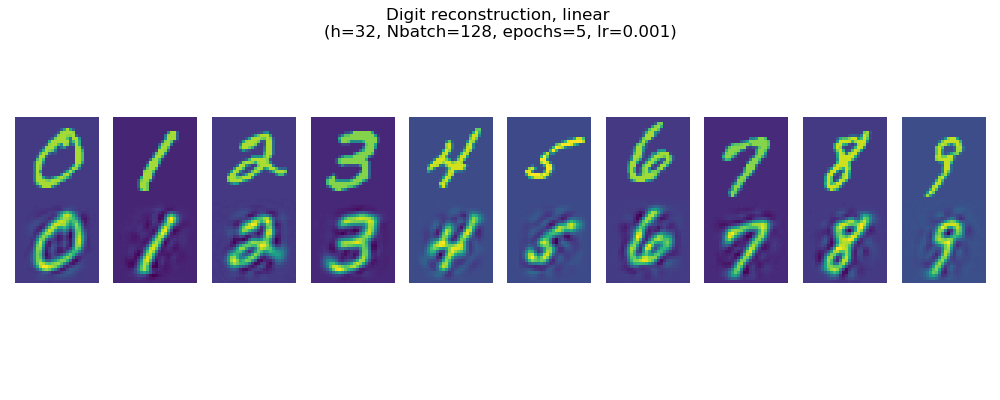
\includegraphics[width=0.47\textwidth]{HW4/HW4_plots/A3a_h32.png} }}\\
        \subfloat[After 5 epochs, with 0.001 learning rate, the test loss is 0.00077228] {{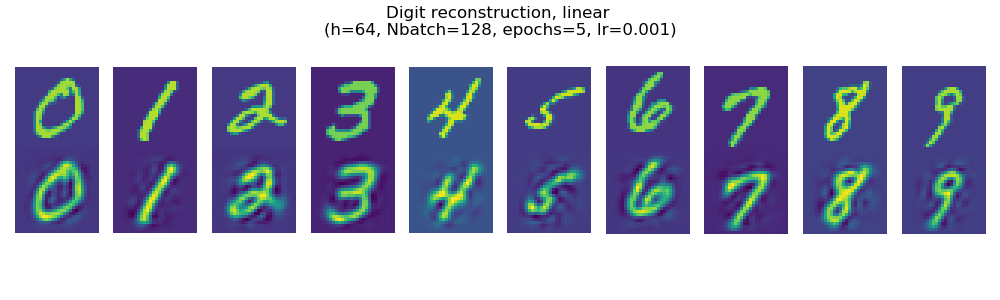
\includegraphics[width=0.47\textwidth]{HW4/HW4_plots/A3a_h64.png} }}\\
        \subfloat[After 5 epochs, with 0.001 learning rate, the test loss is 0.00077527] {{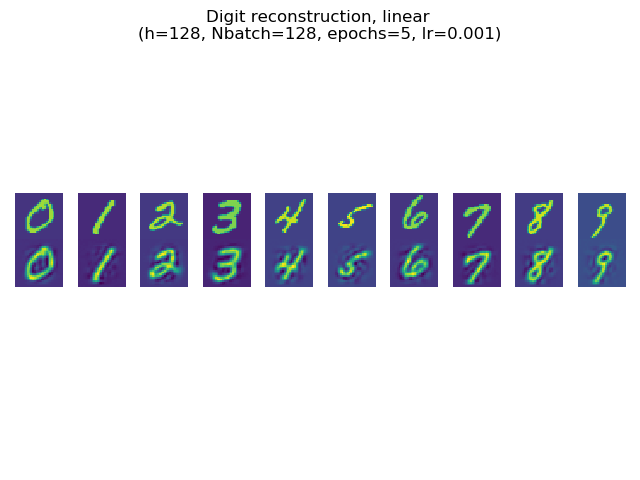
\includegraphics[width=0.47\textwidth]{HW4/HW4_plots/A3a_h128.png} }}
        \caption{MNIST reconstructions using various different hyperparameters.}
    \end{figure}
    
    
    \newpage
    \item \points{10} Use a single-layer network with non-linearity. Let $W_e\in\R^{h\times d}$,$W_d\in\R^{d\times h}$, and activation $\sigma:\R\rightarrow\R$. Given some $x\in\R^d$, the forward pass is formulated as 
    $$\F_2(x) = \sigma(W_d\sigma(W_ex))$$
    Report the same findings as asked for in part a for $h\in\{32,64,128\}$.
    \begin{figure}[h!]
        \centering 
        \subfloat[After 5 epochs, with 0.001 learning rate, the test loss is 0.00221150] {{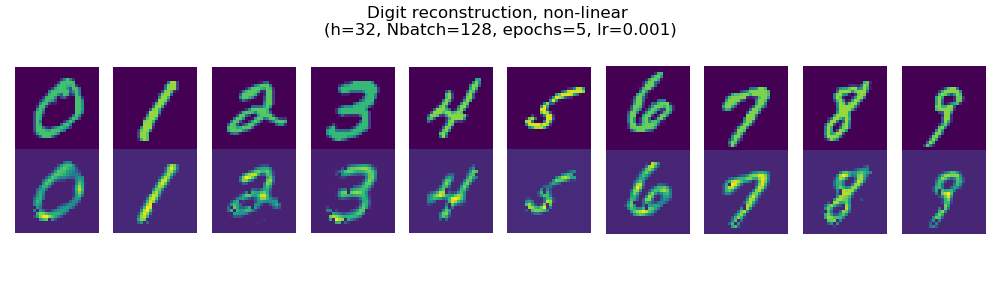
\includegraphics[width=0.47\textwidth]{HW4/HW4_plots/A3b_h32.png} }}\\
        \subfloat[After 5 epochs, with 0.001 learning rate, the test loss is 0.00205961] {{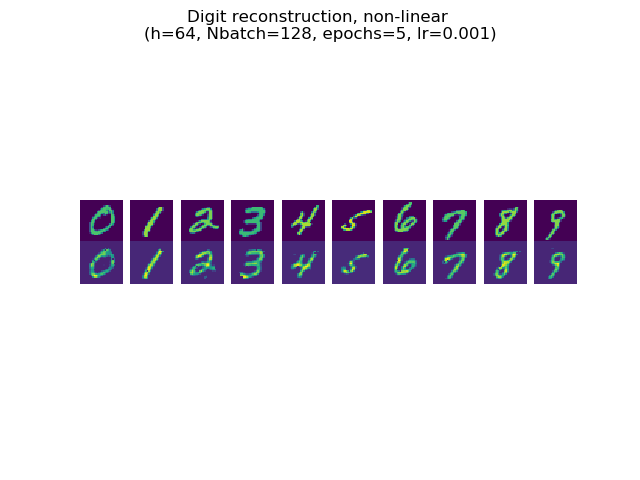
\includegraphics[width=0.47\textwidth]{HW4/HW4_plots/A3b_h64.png} }}\\
        \subfloat[After 5 epochs, with 0.001 learning rate, the test loss is 0.00215065] {{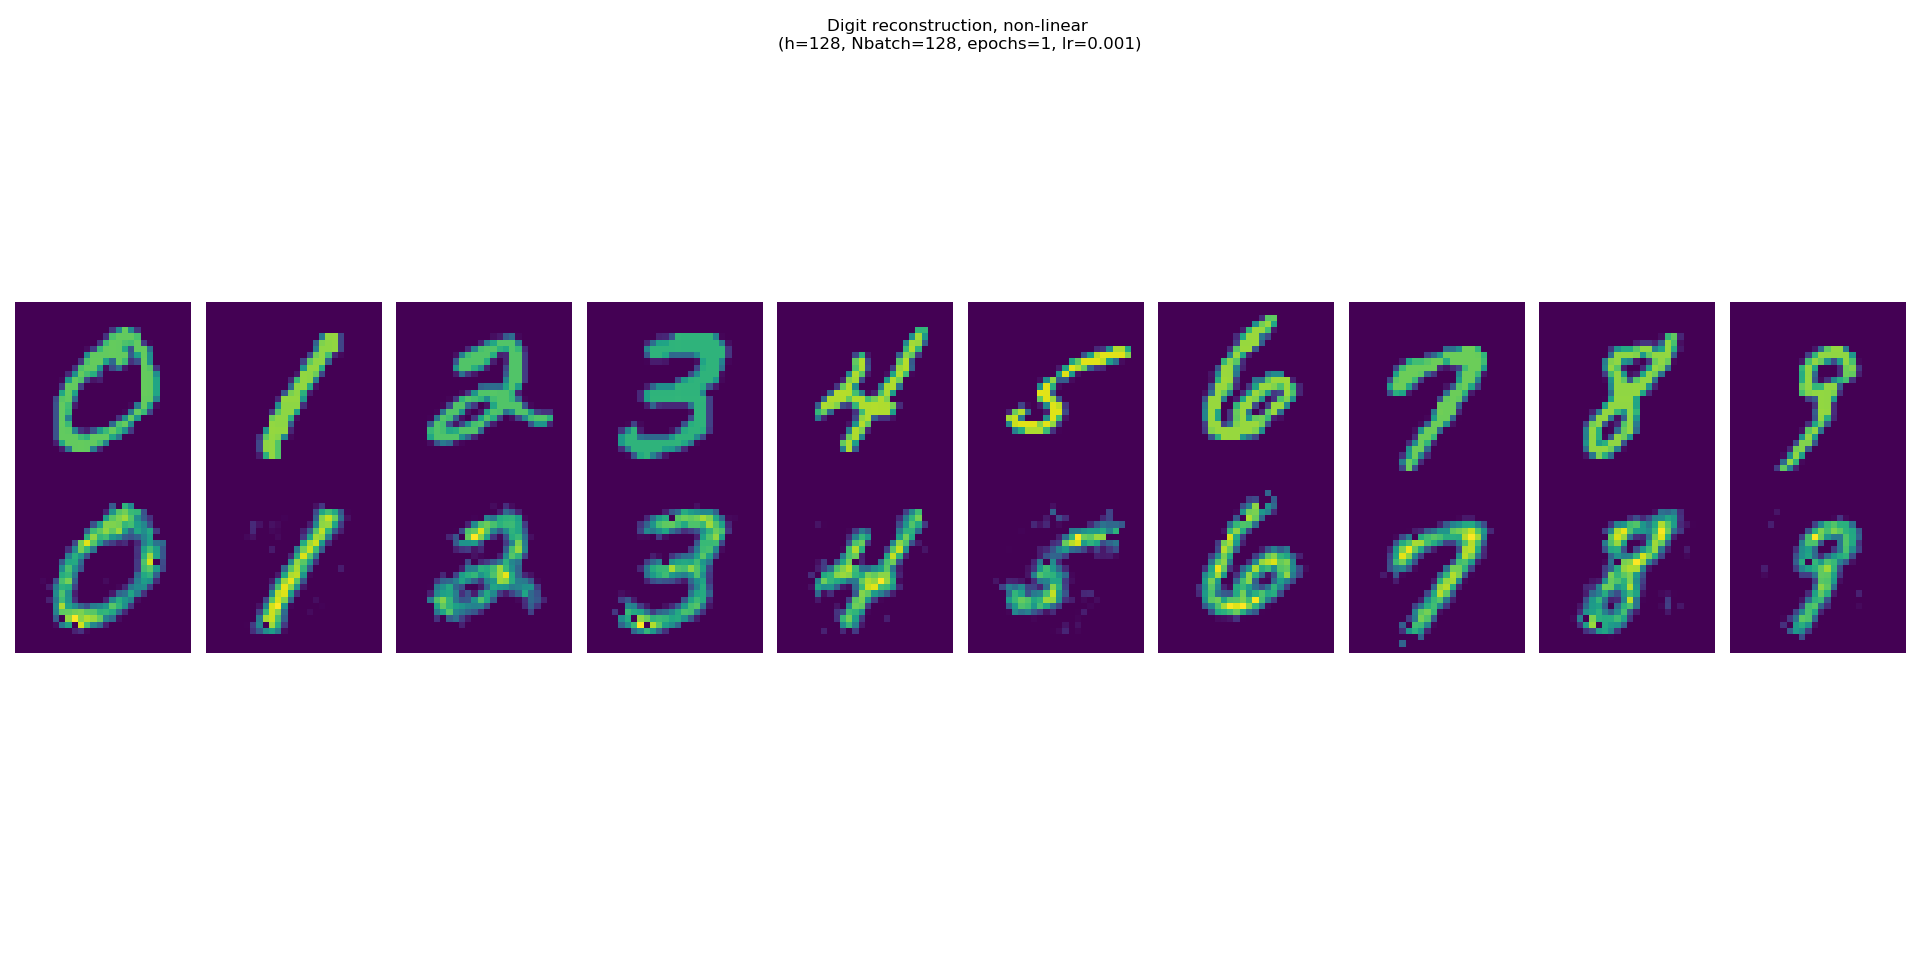
\includegraphics[width=0.47\textwidth]{HW4/HW4_plots/A3b_h128.png} }}
        \caption{MNIST reconstructions using various different hyperparameters.}
    \end{figure}
    
    
    \item \points{5} Now, evaluate $\F_1(x)$ and $\F_2(x)$ (use $h=128$ here) on the test set. Provide the test reconstruction errors in a table.
    \begin{table}[h!]
    \centering
        \begin{tabular}{l|l}
               &  loss   \\
        \hline 
        $\F_1$ &  0.00077527 \\
        \hline 
        $F_2$  & 0.00215065   
        \end{tabular}
    \end{table}
    
    \newpage
    \item \points{5} In a few sentences, compare the quality of the reconstructions from these two autoencoders, compare with those of PCA from last assignment. You may want to re-run your code for PCA using the different $h$ values as the number of top-k eigenvalues. \\
    Effectively it's a poor-mans PCA in this context - we apply some linear transformation to the dataset and then learn the randomly instantiated weights in the decode step to linearly transform the dataset back. It is not surprising that the reconstructions are nearly identical to the input. Statistically, nonlinear reconstruction performs worse than the linear one. Visually, however, the non-linear reconstruction behaves better. This is because our eyes do not notice the missing bright pixel or two but because of the non-linearity we are able to better ignore the background. \\
    Plots below showcase my analogy with a 2-component PCA. I project the image all the way down to 3 dimensional latent space and then plot them against each other. Points are colored according to labels. This neatly shows how autoencoder seems to dis-entangle various digits by grouping them in its latent space, similarly to PCA. 
    \begin{figure}[h!]
        \centering 
        \subfloat{{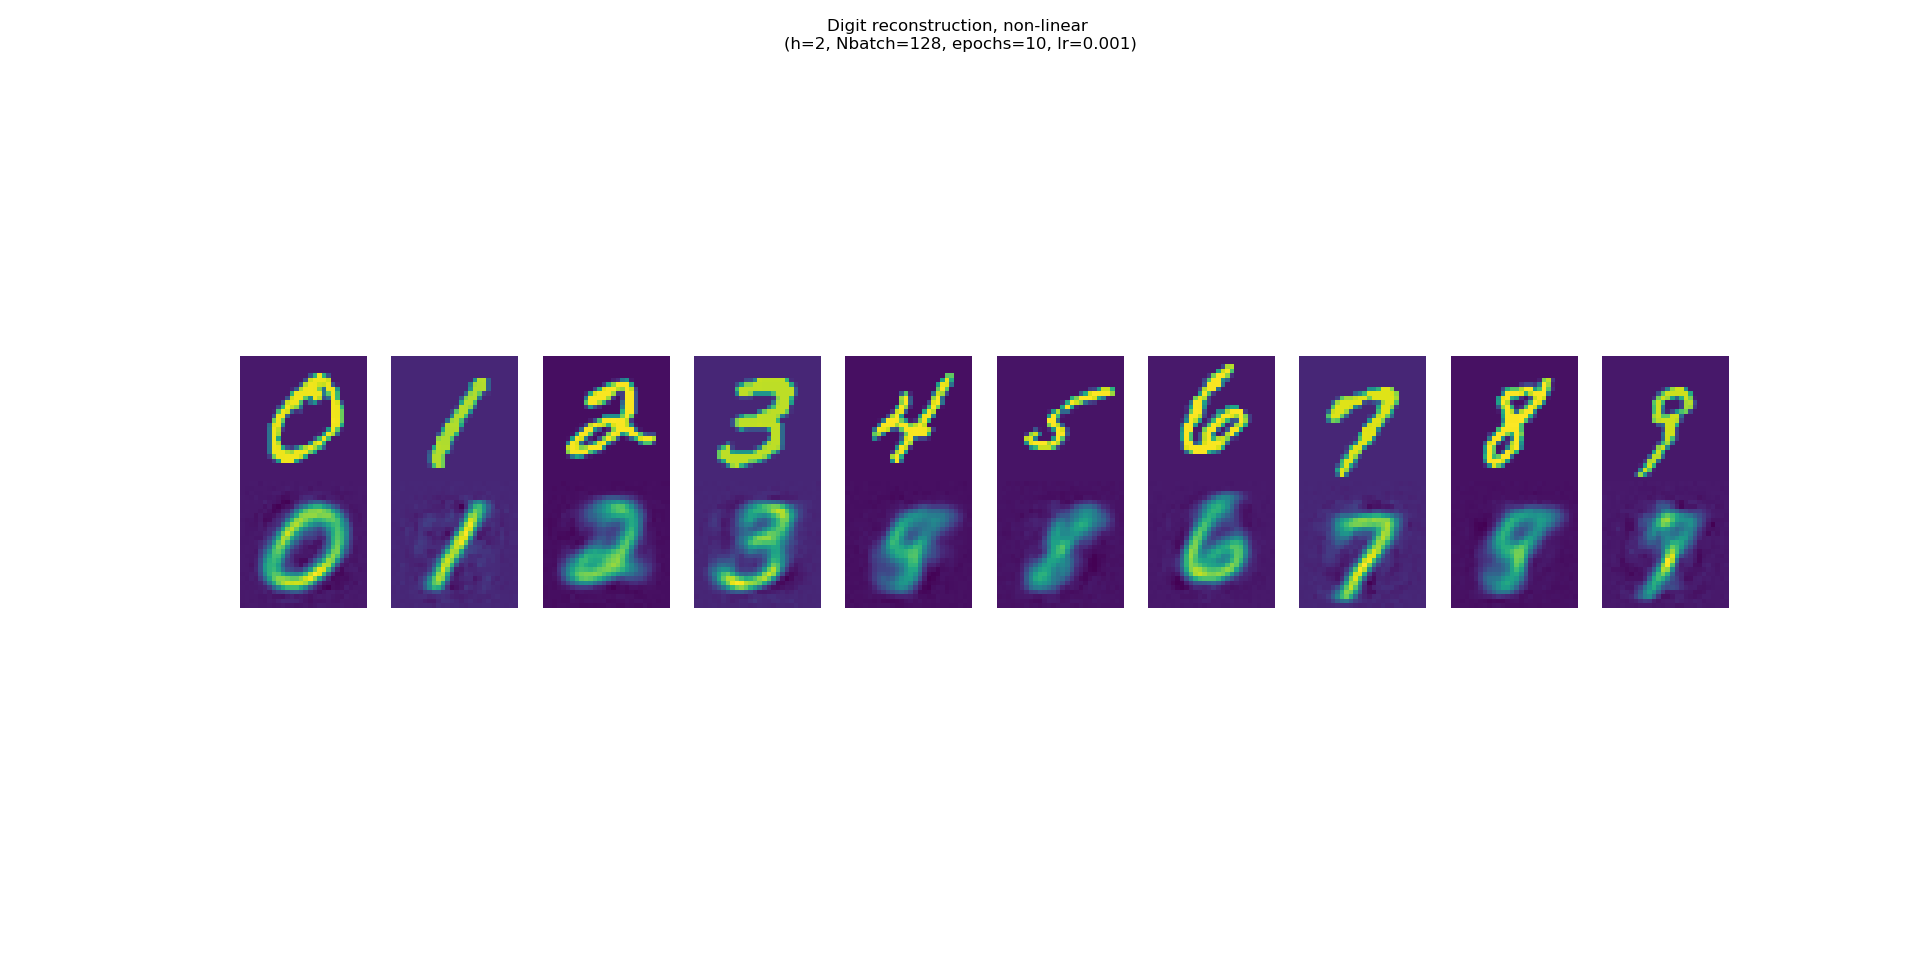
\includegraphics[width=0.47\textwidth]{HW4/HW4_plots/MyAutoencoder_digits.png} }}
        \subfloat{{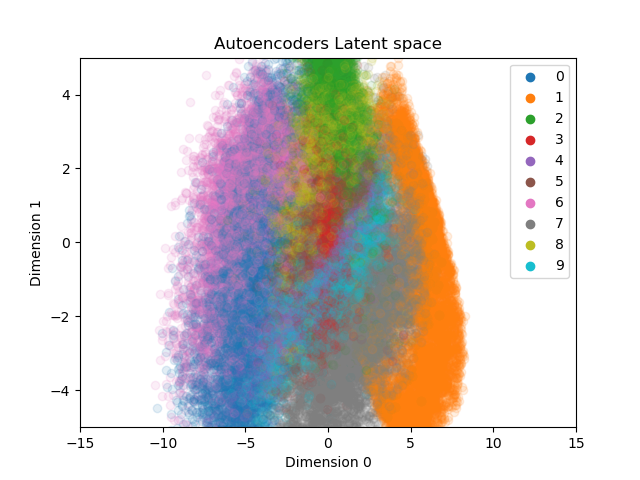
\includegraphics[width=0.47\textwidth]{HW4/HW4_plots/MyAutoencoder_LatentSpace1.png} }} \\
        \subfloat{{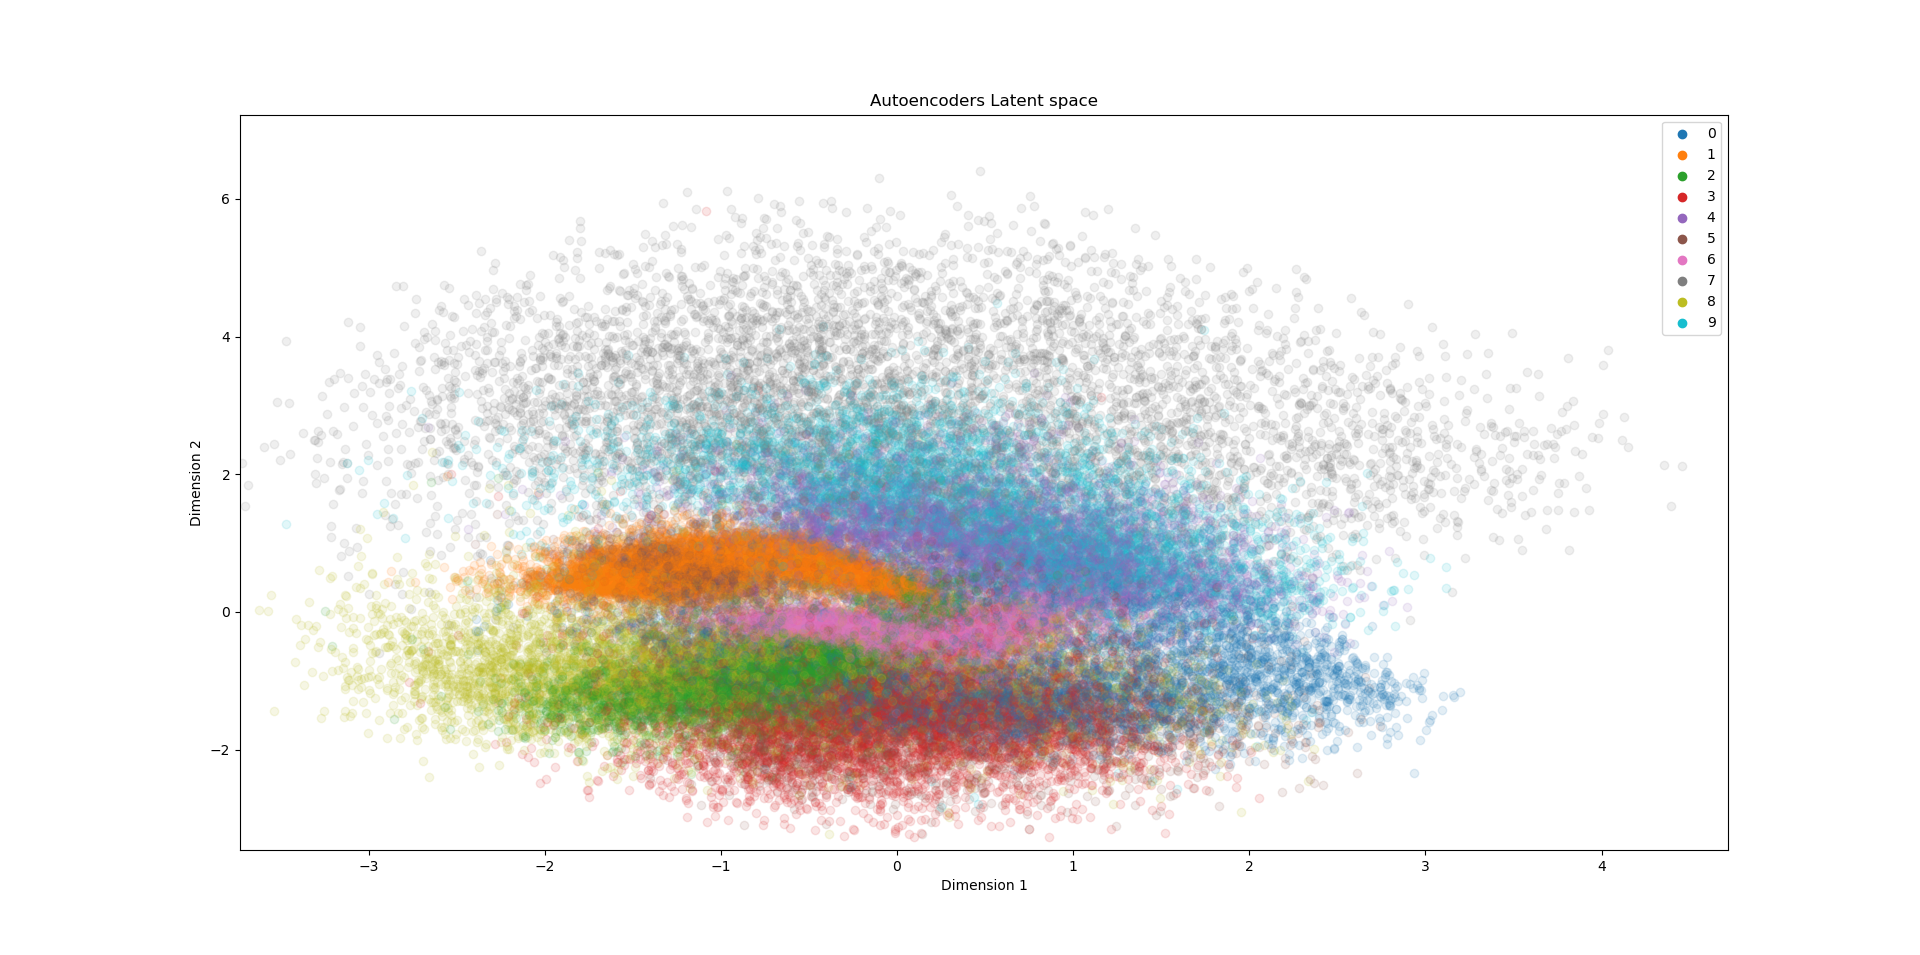
\includegraphics[width=0.47\textwidth]{HW4/HW4_plots/MyAutoencoder_LatentSpace2.png} }}
        \subfloat{{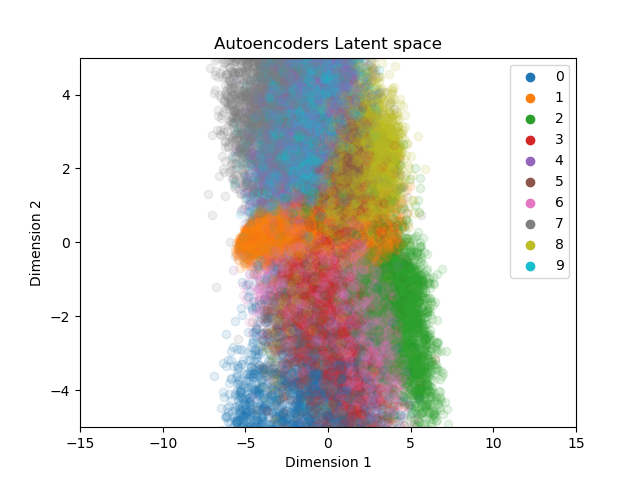
\includegraphics[width=0.47\textwidth]{HW4/HW4_plots/MyAutoencoder_LatentSpace3.png} }}
        \caption{MNIST reconstructions using my autoencoder. They are visually relatively poor, no doubt due to a low-dimensional latent space. Trained for 10 epochs with learning rate at 0.001 the test loss is 0.00039763.}
    \end{figure}
\end{enumerate}
\newpage
\lstinputlisting{HW4_code_solutions/autoencoders.py}  




\newpage
\section*{Unsupervised Learning with Autoencoders}

A5.  In this problem we will explore different deep learning architectures for image classification on the CIFAR-10 dataset. 

For all of the following, apply a hyperparameter tuning method (grid search, random search, etc.) using the validation set, report the hyperparameter configurations you evaluated and the best set of hyperparameters from this set, and plot the training and validation classification accuracy as a function of iteration. Produce a separate line or plot for each hyperparameter configuration  evaluated.  Finally, evaluate your best set of hyperparameters on the test data and report the accuracy. On the larger networks, you should expect to tune hyperparameters and train to at least 70\% accuracy. Here are the network architectures you will construct and compare.
\begin{enumerate}
    \item \points{15} Fully-connected output, 0 hidden layers (logistic regression): this network has no hidden layers and linearly maps the input layer to the output layer.
    \begin{figure}[h!]
        \centering 
        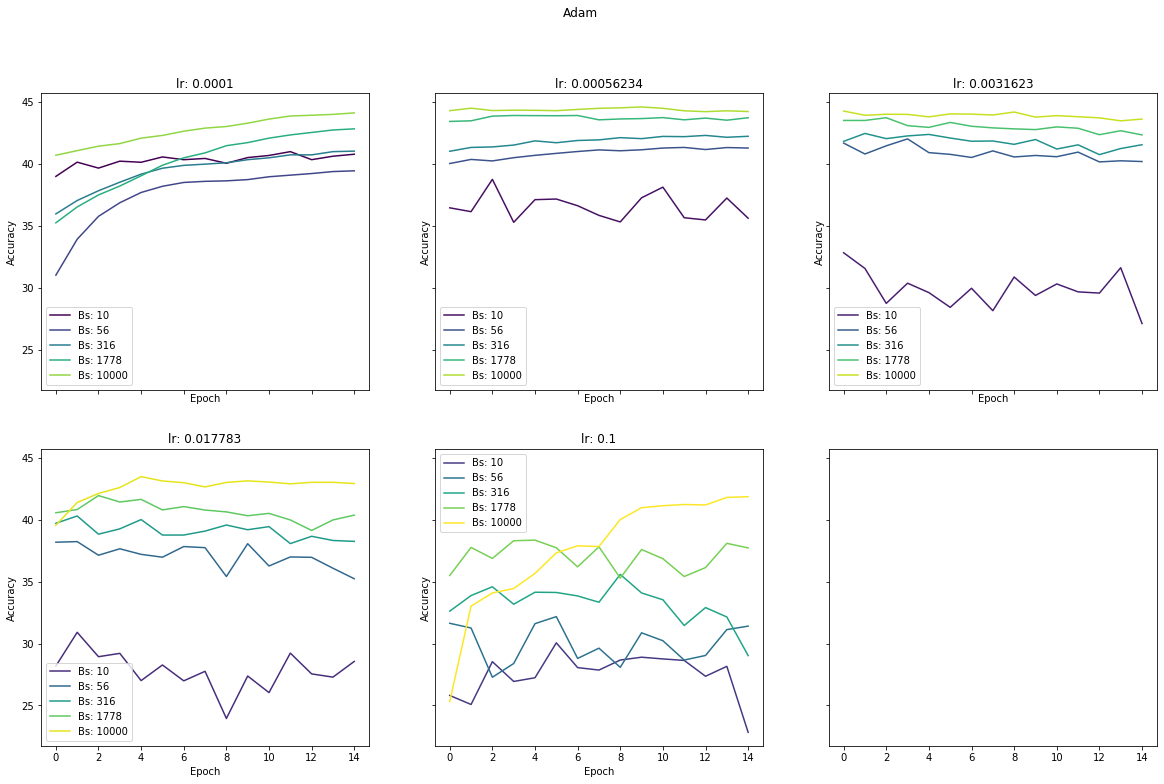
\includegraphics[width=0.47\textwidth]{HW4/HW4_plots/A5a.png}
    \end{figure}
    \begin{figure}
    \centering
        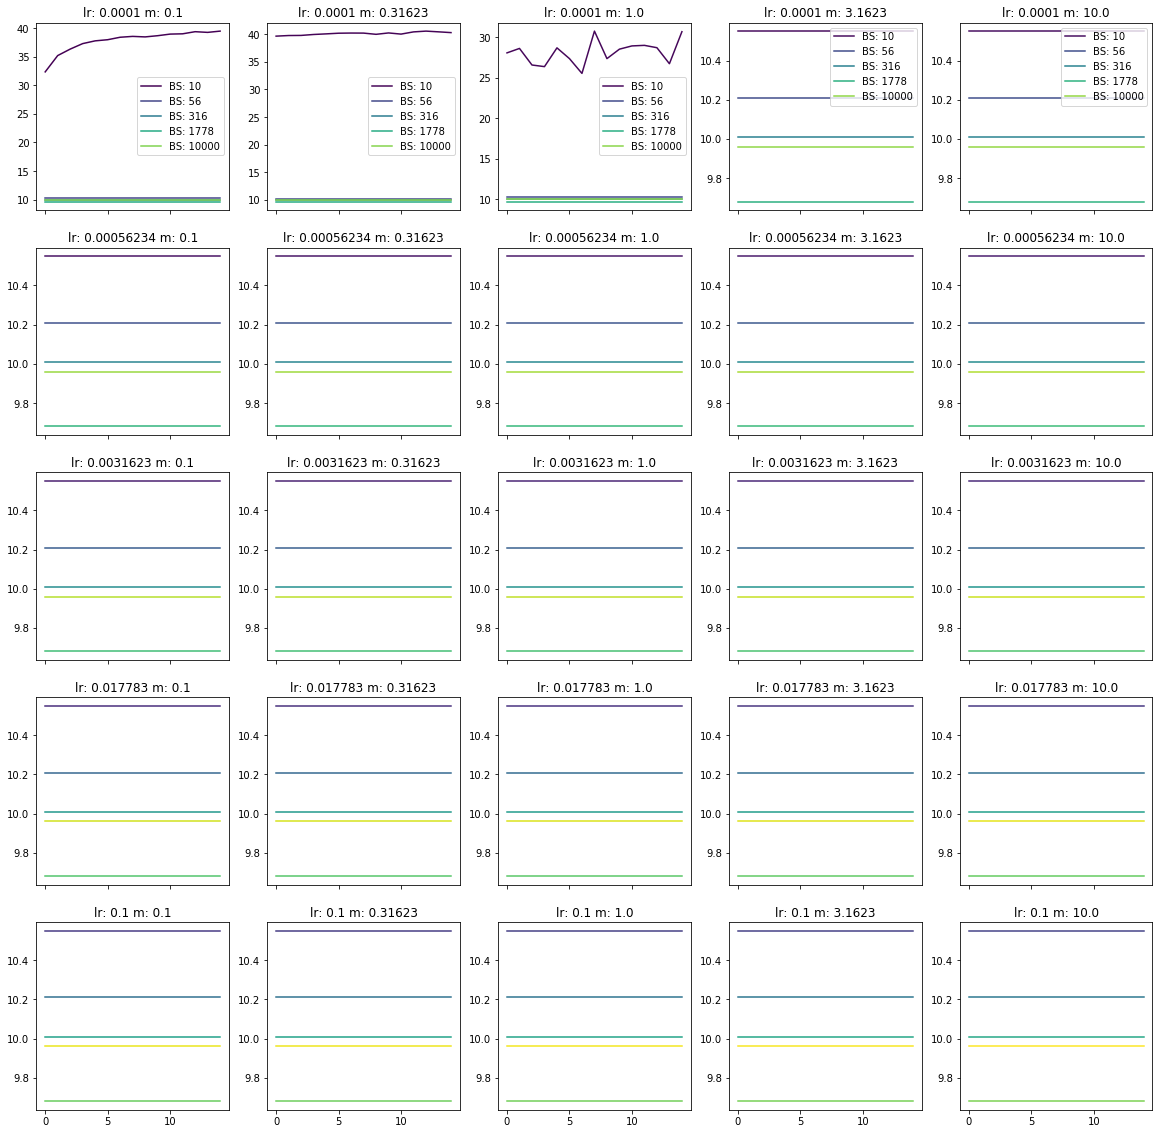
\includegraphics[width=0.85\textwidth]{HW4/HW4_plots/A5a1.png}
        \caption{SGD optimizer}
    \end{figure}
    \newpage
    \item \points{15} Fully-connected output, 1 fully-connected hidden layer: this network has one hidden layer denoted. M will be a hyperparameter you choose (M could be in the hundreds). The non linearity applied to the hidden layer will be the relu.
    \item \points{15} Convolutional layer with max-pool and fully-connected output.
    \item Tuning: Return to the original network you were left with at the end of the tutorial Training a classifier. Tune the different hyperparameters (number of convolutional filters, filter sizes, dimensionality of the fully-connected layers, step size, etc.) and train for a sufficient number of iterations to achieve a test accuracy of at least 70\%. Provide the hyperparameter configuration used to achieve this performance.
\end{enumerate}

This code produced the above plots and contains the code for the remaining solutions. I ran into a problem with the grid\_search implementation because I opted to use the GPUs to speed up the process. If you look at the SGD plots they are not correct after the first iteration. Running the sampling (commented out code at the end) for the same parameters I get different results than the ones that actually get saved. I don't know hwere the problem is. It obviously should not be constant accuracy across the epoch (and as I said, when I run that sampling manually it isn't) but when I run the A5a sampler then suddenly it is. I've struggled for two days trying to fix that problem but haven't been able to figure out where the problem is. I'm out of time so I'm submitting what I have. The are different when run out of the loop, but in it they all end up being the same. Running on CPU took 558 minutes (9.3 hours) for A5a which means it's just not possible for me to finish this on time unless I run on GPU (about 1.5hours on a Tesla). Hopefully it'll count for some points at least. Things to note from manual runs is that SGD seems to perform better on smaller batches (because averaging over many points tends to get it stuck in some local minima whereas jumps are more erratic on smaller batch sizes) and Adam seems to perform as expected. It's not too difficult to reach 70\% accuracy in those cases for enough epochs. 
\lstinputlisting{HW4_code_solutions/cifar.py}  




\end{document}